\section{Background estimation technique}
\label{sec:alpha}

The goal of the analysis is to look for localised excesses in the \mtVZ spectrum. The \emph{$\alpha$-method} is used in searches for heavy resonances since the LHC Run 1~\cite{Khachatryan:2015cwa}, and it has been introduced to be less dependent on the MC simulation for the background \mtVZ estimation, due to the many sources of systematic uncertainties that are hard to understand and control. The two exclusive regions, \emph{signal region} (SR) and \emph{sidebands region} (SB), define a signal enriched or signal depleted phase space, respectively. First, the background normalization is extracted from data in the SB. Then, the $\alpha$-method extracts a predicted shape from the data in the SB to the SR using a transfer function (the $\alpha$ function) derived from simulation. The method relies on the assumption that the correlation between \mtVZ and the groomed jet mass is reasonably well reproduced by the MC. The $\alpha$ ratio is deemed to be more trustworthy since many systematic uncertainties would approximately cancel in the ratio.

{\color{red} EXPLAIN WHY Z+jet and W+jet are together}

\noindent The $\alpha$ function is defined as the ratio of the two functions describing the simulated \mtVZ shape in the SR and SB:
%In the simplest case, only one dominant background is present. 
$$\alpha(\mtVZ) = \frac{N_{\text{SR}}^{\text{MC,bkg}}(\mtVZ)}{N_{\text{SB}}^{\text{MC,bkg}}(\mtVZ)}$$
%
and the background distribution in the SR is thus estimated as the product of  $\alpha(\mtVZ)$ with the shape in the data SB:
%
$$N_{\text{bkg}}(\mtVZ) = N_{\text{SB}}(\mtVZ) \times \alpha(\mtVZ)$$
%
Notice that in the above description does not include the definition of the SB and SR. Ideally, the best choice would be a variable such that the distribution of \mtVZ in the Signal and Sideband regions are similar. In this analysis, the softdrop+PUPPI corrected jet mass $m_j$ (see Section~\ref{ssec:jetmass}) is chosen as the control variable, and the cut values are those reported in Section~\ref{ssec:massopt}. All the selections used in the $\alpha$ method background prediction are the same reported in Section~\ref{sec:selections}.
In order to respect the blinding policy of the diboson VV searches, the Higgs mass window is not used neither for the background estimation (it can be potentially contamined by a signal) nor as signal region.

In a real case scenario, the background is not purely composed of one single process neither in the SR nor in the SB. The background composition is assumed to be dominated by one single process (\V+jets) whose modeling in simulation is considered not to be trustworthy. Other subdominant backgrounds (\ttbar and single-t production (Top), and \V\V) generally have smaller contributions (of the order of 5\% for \V\V, and 9\% for Top) , and are considered quite well understood and modeled by MC generators. 

{\color{red} EXPLAIN WHY Z+jet and W+jet are together}

The shape and normalization of the diboson and Top production is taken from the simulation.
The sub-dominant backgrounds are then subtracted from the \V+jets contribution when fitting this template to data.

%One single $\alpha$ function is defined for each channel and category, that is obtained with the simulated background composition, and multiplied by the data distribution in the SB. This implies that the shape change between SB and SR does not heavily depend on the background process, and even if it does, the $\alpha$ function is already built with the expected ratio between various processes. With respect to the subtraction of the sub-dominant background, this choice has the advantage to take into account the shape variation also for the sub-dominant backgrounds, which can be non-negligible in some channels. Anyway, the normalization for the sub-dominant backgrounds is estimated separately due to the different jet mass distribution.

A different background prediction is derived for each category separately, thus dividing low- and high-purity categories, and it is calculated in a transverse mass range $950 <$ \mtVZ $<4750$ GeV.

\subsection{Background normalization}\label{ssec:alphaNorm}

The first step in the background prediction consists in a proper estimation of the background normalization. The three main backgrounds (\V+jets, Top, and VV) are considered separately due to the different shape in the jet mass distribution. The three contributions are described with functional forms determined by fits on the simulated backgrounds.
%The so-built templates are summed together, maintaining the relative weights between the three, and finally fitted to the data in the jet mass sidebands. The integral of the fitted function over the SR jet mass range represents the background normalization in the SR.
The number of expected events in the SR is extracted through the same equation:
$$N_{SR}^{data} = \left[ N_{SB}^{data} - N_{SB}^{Top} - N_{SB}^{VV} \right] \times \left[ \frac{N_{SR}^{Vjet}}{N_{SB}^{Vjet}} \right]  + N_{SR}^{Top} + N_{SR}^{VV}$$
where in this case $N$ are the number of events, and not functions.

The empirical functional forms for each background are chosen to reflect the physics properties of the samples. In the low-purity category, the \V+jets background is a falling background with no peaks, modelled as a power law, while in the high-purity category the \V+jets background component is characterized by a broad distribution roughly centered at $m_\V$, modelled as a gaussian, with an exponential tail at high mass values. The exponential falling VV $m_j$ spectrum shows a peak, corresponding to the vector boson hadronic decay reconstruction, that is modelled as a gaussian. For the jet mass spectrum of the Top backgrounds, the peaks corresponding to the $W$ and top mass can be modelled as gaussian functions, superimposed to a falling exponential background.

%The empirical functional forms for each background are chosen to reflect the physics properties of the samples. 
%In the low-purity category, the \V+jets background has a falling background with no peaks, while in the high-purity category the \V+jets background component is characterized by a broad distribution roughly centered at $m_\V$, with an exponential tail at high mass values.

%On top of the jet mass spectrum, the VV has one peak, corresponding to the vector boson hadronic decay reconstruction.
%% , and possibly a second one due to the presence of the Higgs. In certain channels, the latter is not visible due to the smaller cross section with respect to the former. 
%For the Top background the jet mass spectrum is similar to the V+jet one, with a falling behaviour for the low-purity category, and broader distribution roughly peaked at $m_\V$ and with the exponential tail at high mass for the high-purity categories.
The functional forms chosen to build the jet mass templates are:

\begin{itemize}
  %\item[{\bf Exp}:] an exponential function: $$F_{\rm Exp}(x)=e^{ax}$$
  %\item[{\bf Pol}:] a third order polynomial: $$F_{\rm Pol}(x)=a_0 \cdot x + a_2 \cdot x^2 + a_3 \cdot x^3 $$
  \item[{\bf ErfExp}:] an ``error function'', that consists of an exponential multiplied by an Erf: $$F_{\rm ErfExp}(x)=e^{ax} \cdot \frac{1 + {\rm Erf}((x-b)/w)}{2}$$
  \item[{\bf ErfExpTail}:] an ErfExp modified to account for an additional term in the exponential: $$F_{\rm ErfExpTail}(x)=e^{-x/(a+b*x)} \cdot \frac{1 + {\rm Erf}((x-o)/w)}{2}$$
  \item[{\bf ErfPow2}:] an Erf multiplied by a power law: $$F_{\rm ErfPow2}(x)={ \left( \frac{x}{\sqrt{s}} \right)}^{- c_0 + c_1 \log(x/\sqrt{s})} \cdot \frac{1 + {\rm Erf}((x-o)/w)}{2}$$
  %
  %\item[{\bf Gaus}:] one gaussian: $$F_{\rm Gaus}(x) = \cdot e^{2(x-a)^2/b}$$
  %\item[{\bf Gaus2}:] two gaussians: $$F_{\rm Gaus2}(x) = f_0 \cdot e^{2(x-a)^2/b} + (1-f_0) \cdot e^{2(x-c)^2/d}$$
  \item[{\bf Gaus3}:] three gaussians: $$F_{\rm Gaus3}(x) = f_0 \cdot e^{2(x-a)^2/b} +f_1 \cdot e^{2(x-c)^2/d} + (1-f_0-f_1) \cdot e^{2(x-e)^2/g}$$
  %
  \item[{\bf ExpGaus}:] an exponential plus one gaussian: $$F_{\rm ExpGaus}(x) = f_0 \cdot e^{ax} + (1-f_0) \cdot e^{2(x-b)^2/c}$$
  %\item[{\bf ExpGaus2}:] an exponential plus two gaussians: $$F_{\rm ExpGaus2}(x) = f_0 \cdot e^{ax} + f_1 \cdot e^{2(x-b)^2/c} + (1-f_0-f_1) \cdot e^{2(x-d)^2/e}$$
  \item[{\bf ErfExpGaus}:] an error function plus one gaussian: $$F_{\rm ErfExpGaus}(x) = f_0 \cdot F_{\rm ErfExp}(x,a,b,c) + (1-f_0) \cdot e^{2(x-d)^2/e}$$
  \item[{\bf ErfExpGaus2}:] an error function plus two gaussians: $$F_{\rm ExpGaus2}(x) = f_0 \cdot F_{\rm ErfExp}(x,a,b,c) + f_1 \cdot e^{2(x-d)^2/e} + (1-f_0-f_1) \cdot e^{2(x-f)^2/g}$$
\end{itemize}

The choice of the functions is channel-dependent, and it depends on the background shape and the available statistics, and is summarized in Table~\ref{tab:MassFunctions}.

\begin{table}[!htb]
  \begin{center}
    \begin{tabular}{cc|ccccc}
      \multicolumn{2}{c}{category} & \V+jets & alt. \V+jets & Top & VV \\
      \hline
      & $2\nu$, low-purity  & ErfPow2 & ExpGaus & ErfExpGaus2 & ExpGaus \\
      \hline
      & $2\nu$, high-purity & ExpGaus & ErfExpGaus & ErfExpGaus2 & ExpGaus \\
      \hline
    \end{tabular}
  \end{center}
  \caption{Chosen functions to fit the jet mass distribution for each channel.}\label{tab:MassFunctions}
\end{table}

The following plots (Figure~\ref{fig:XVZnn_JetMass}-\ref{fig:XVZnn_JetMass}) show the mass fits to the jet mass in the different channels. Table~\ref{tab:BkgNorm} summarizes the expected background yield in the signal region, that is in agreement with observation in both the purity categories.

%[FIXME: numbers in table to be updated]

\begin{table}[!htb]
  \begin{center}
    \begin{tabular}{cc|cccccc}
      region & category   & Expected  & Stat.       & Syst.      & Alt. function & Observed \\
      \hline
      SB     & low-purity & $2356.6$ & $\pm 52.5$ & $\pm 16.0$ & $\pm 1.1$    & $2314$ \\
      SR     & low-purity & $1093.2$  & $\pm 48.1$ & $\pm 16.4$ & $\pm 49.1$   & $1153$ \\
      \hline
      SB & high-purity    & $779.8$  & $\pm 29.1$ & $\pm 13.1$ & $\pm 0.3$  & $774$ \\
      SR & high-purity    & $254.4$  & $\pm 15.3$ & $\pm 17.9$ & $\pm 7.8$  & $271$ \\
      \hline
    \end{tabular}
  \end{center}
  \caption{Expected background yield in the SB ($30 < m_j < 65\GeV$, $m_j > 135\GeV$ )and in the SR ($65 < m_j < 105\GeV$) and relative uncertainties.}\label{tab:BkgNorm}
\end{table}

\clearpage


%%% 2 electrons %%%

\begin{figure}[!htb]
  \centering
    \includegraphics[width=.32\textwidth]{v9/plotsAlpha/XVZnnlp/VjetMass.pdf}
    \includegraphics[width=.32\textwidth]{v9/plotsAlpha/XVZnnlp/VVMass.pdf}
    \includegraphics[width=.32\textwidth]{v9/plotsAlpha/XVZnnlp/TopMass.pdf}
  \caption{Fit to the simulated $m_j$ in the low-purity category for the three backgrounds: \V+jets (left), VV (center), Top (right). For the main background prediction, the alternative function is displayed with a dotted red line, superimposed to the main choice (continuous light blue curve).}
  \label{fig:XVZnnlp_JetMass}
\end{figure}


\begin{figure}[!htb]
  \centering
    \includegraphics[width=.32\textwidth]{v9/plotsAlpha/XVZnnhp/VjetMass.pdf}
    \includegraphics[width=.32\textwidth]{v9/plotsAlpha/XVZnnhp/VVMass.pdf}
    \includegraphics[width=.32\textwidth]{v9/plotsAlpha/XVZnnhp/TopMass.pdf}
  \caption{Fit to the simulated $m_j$ in the high-purity category for the three backgrounds: \V+jets (left), VV (center), Top (right). For the main background prediction, the alternative function is displayed with a dotted red line, superimposed to the main choice (continuous light blue curve).}
  \label{fig:XVZnnhp_JetMass}
\end{figure}


\begin{figure}[!htb]
  \centering
    \includegraphics[width=.495\textwidth]{v9/plotsAlpha/XVZnnlp/XVZnnlp_JetMass_U.pdf}
    \includegraphics[width=.495\textwidth]{v9/plotsAlpha/XVZnnhp/XVZnnhp_JetMass_U.pdf}
  \caption{Fit to data $m_j$ in the low- (left) and high-purity category (right).}
  \label{fig:XVZnn_JetMass}
\end{figure}




\clearpage




\subsection{Background shape}\label{ssec:alphaShape}

The mass of the resonance candidate (\mtVZ) is parametrized separately for the V+jets ($N_{SR}^{Vjet}(\mtVZ)$, $N_{SB}^{Vjet}(\mtVZ)$), Top production  ($N_{SR}^{Top}(\mtVZ)$, $N_{SB}^{Top}(\mtVZ)$), and dibosons ($N_{SR}^{VV}(\mtVZ)$, $N_{SB}^{VV}(\mtVZ)$). These functions are extracted fitting the simulated \mtVZ spectra in SR and SB, respectively. The top and the diboson are normalized to luminosity. The V+jets functions are used to extract the $\alpha$-function: $$\alpha(\mtVZ) = \frac{N_{SR}^{Vjet}(\mtVZ)}{N_{SB}^{Vjet}(\mtVZ)}$$

The main background is extracted through a fit to data in the SB, after subtracting the corresponding the Top and VV contribution from data. The resulting shape is then multiplied by the $\alpha$-function in order to get the main background expectation in the SR. Finally, the Top and diboson contribution in the SR is added to the main background estimation.

In formulas, the procedure used to extract the total background prediction is the following:

$$N_{SR}^{main}(\mtVZ) = N_{SR}^{main}(\mtVZ) \times \alpha(\mtVZ)$$

$$N_{SR,SB}^{bkg}(\mtVZ) = N_{SR,SB}^{main}(\mtVZ) + N_{SR,SB}^{Top}(\mtVZ) + N_{SR,SB}^{VV}(\mtVZ)$$

$$N_{SR}^{data}(\mtVZ) = \left[ N_{SB}^{data}(\mtVZ) - N_{SB}^{Top}(\mtVZ) - N_{SB}^{VV}(\mtVZ) \right] \times \left[ \frac{N_{SR}^{Vjet}(\mtVZ)}{N_{SB}^{Vjet}(\mX)} \right]  + N_{SR}^{Top}(\mtVZ) + N_{SR}^{VV}(\mtVZ) $$

The functions used to parametrize the \mtVZ distributions are:

\begin{itemize}
  %\item[{\bf Exp}:] a simple exponential function. Its simplicity is balanced by the limited possibility to model the \mtVZ tails in some channels: $$F_{\rm Exp}(x) = e^{ax}$$
  %\item[{\bf Exp2}:] a double exponential function. It has better description of the tails, but introduces two new parameters: $$F_{\rm Exp2}(x) = (1-f_0) \cdot e^{ax} + f_0 \cdot e^{bx}$$
  \item[{\bf ExpN}:] a product of two exponentials: $$F_{\rm ExpN}(x) = e^{ax+b/x}$$
  %\item[{\bf ExpN2}:] a product of three exponentials: $$F_{\rm ExpN2}(x) = e^{ax+b/x+c/x^2}$$
  \item[{\bf ExpTail}:] a modified exponential function with an additional parameter to model the exponential tails: $$F_{\rm ExpTail}(x) = e^{-x/(a+bx)}$$
  %\item[{\bf ExpTail2}:] a modified exponential function with two additional parameters to model the exponential tails and turn-on: $$F_{\rm ExpTail}(x) = e^{-x/(a+bx)+c/x^2}$$
  %\item[{\bf ErfExpN}:] an ExpN multiplied by an error function to describe potential ``turn-on'' effects: $$F_{\rm ExpN}(x) = e^{ax+b/x} \cdot \frac{1 + {\rm Erf}((x-b)/w)}{2}$$
  %\item[{\bf ErfExpTail}:] an ExpTail multiplied by an error function to describe potential ``turn-on'' effects: $$F_{\rm ExpTail}(x) = e^{-x/(a+bx)}\cdot \frac{1 + {\rm Erf}((x-b)/w)}{2}$$
  %\item[{\bf Pow}:] a second-order power function: $$F_{\rm Pow}(x) = a_0 \cdot x + a_1 \cdot x^2$$
\end{itemize}

The functions chosen to parametrize the main background and extract the $\alpha$-function are reported in Table~\ref{tab:XMassFunctions} for each category.

As a cross-check for the main $\alpha$-function used in the background estimation, an additional $\alpha$-function is extracted with alternative function choices. Table~\ref{tab:XMassFunctions} reports both the main function and the alternative function.

\begin{table}[!htb]
  \begin{center}
    \begin{tabular}{cc|cccccc}
      \multicolumn{2}{c}{category} & Main bkg function & Main bkg alternative & diboson & top \\
      \hline
       & $2\nu$, low-purity  & ExpN & ExpTail & ExpTail & ExpTail \\
      \hline
       & $2\nu$, high-purity  & ExpTail & ExpN & ExpTail & ExpTail \\
      \hline
    \end{tabular}
  \end{center}
  \caption{Main and alternative functions chosen to parametrize the main background contribution in the \mtVZ distribution for each channel.}\label{tab:XMassFunctions}
\end{table}



\clearpage

%%% 2 neutrinos %%%

\begin{figure}[!htb]
  \centering
    \includegraphics[width=.32\textwidth]{v9/plotsAlpha/XVZnnlp/VjetSB.pdf}
    \includegraphics[width=.32\textwidth]{v9/plotsAlpha/XVZnnlp/VVSB.pdf}
    \includegraphics[width=.32\textwidth]{v9/plotsAlpha/XVZnnlp/TopSB.pdf}
    \caption{2 neutrinos, low-purity channel. Fits to the simulated background components \V+jets (left), VV (center), Top (right) in the sidebands (SB).}
  \label{fig:XVZnnlp_SB}
\end{figure}

\begin{figure}[!htb]
  \centering
    \includegraphics[width=.32\textwidth]{v9/plotsAlpha/XVZnnlp/VjetSR.pdf}
    \includegraphics[width=.32\textwidth]{v9/plotsAlpha/XVZnnlp/VVSR.pdf}
    \includegraphics[width=.32\textwidth]{v9/plotsAlpha/XVZnnlp/TopSR.pdf}
    \caption{2 neutrinos, low-purity channel. Fits to the simulated background components \V+jets (left), VV (center), Top (right) in the signal region (SR).}
  \label{fig:XVZnnlp_SR}
\end{figure}

\begin{figure}[!htb]
  \centering
    \includegraphics[width=.32\textwidth]{v9/plotsAlpha/XVZnnlp/BkgSB.pdf}
    \includegraphics[width=.32\textwidth]{v9/plotsAlpha/XVZnnlp/AlphaRatio.pdf}
    \includegraphics[width=.32\textwidth]{v9/plotsAlpha/XVZnnlp/AlphaMethod.pdf}
  \caption{2 neutrinos, low-purity channel. Fit to data in the SB (left), alpha function (center), and alpha function compared to the background shape in both SB and SR (right). The black line, with the corresponding $1\sigma$ (green) and $2\sigma$ (yellow) uncertainty bands, represents the $\alpha$-function. The gray line is the alternative $\alpha$-function. The blue and lines represent the estimated background in the SB and SR, respectively, with both the main (solid line) and alternative (dotted line) parametrization.}
  \label{fig:XVZnnlp_Alpha}
\end{figure}


\begin{figure}[!htb]
  \centering
    \includegraphics[width=.32\textwidth]{v9/plotsAlpha/XVZnnhp/VjetSB.pdf}
    \includegraphics[width=.32\textwidth]{v9/plotsAlpha/XVZnnhp/VVSB.pdf}
    \includegraphics[width=.32\textwidth]{v9/plotsAlpha/XVZnnhp/TopSB.pdf}
    \caption{2 neutrinos, high-purity channel. Fits to the simulated background components \V+jets (left), VV (center), Top (right) in the sidebands (SB).}
  \label{fig:XVZnnhp_SB}
\end{figure}

\begin{figure}[!htb]
  \centering
    \includegraphics[width=.32\textwidth]{v9/plotsAlpha/XVZnnhp/VjetSR.pdf}
    \includegraphics[width=.32\textwidth]{v9/plotsAlpha/XVZnnhp/VVSR.pdf}
    \includegraphics[width=.32\textwidth]{v9/plotsAlpha/XVZnnhp/TopSR.pdf}
    \caption{2 neutrinos, high-purity channel. Fits to the simulated background components \V+jets (left), VV (center), Top (right) in the signal region (SR).}
  \label{fig:XVZnnhp_SR}
\end{figure}

\begin{figure}[!htb]
  \centering
    \includegraphics[width=.32\textwidth]{v9/plotsAlpha/XVZnnhp/BkgSB.pdf}
    \includegraphics[width=.32\textwidth]{v9/plotsAlpha/XVZnnhp/AlphaRatio.pdf}
    \includegraphics[width=.32\textwidth]{v9/plotsAlpha/XVZnnhp/AlphaMethod.pdf}
  \caption{2 neutrinos, high-purity channel. Fit to data in the SB (left), alpha function (center), and alpha function compared to the background shape in both SB and SR (right). The black line, with the corresponding $1\sigma$ (green) and $2\sigma$ (yellow) uncertainty bands, represents the $\alpha$-function. The gray line is the alternative $\alpha$-function. The blue and lines represent the estimated background in the SB and SR, respectively, with both the main (solid line) and alternative (dotted line) parametrization.}
  \label{fig:XVZnnhp_Alpha}
\end{figure}

\clearpage


\subsection{Background prediction}
Fig.~\ref{fig:XVZnn_Exp} summarizes the final background predictions as a function of the search variable, the transverse mass. Data and predictions are in agreement in both channels.

\begin{figure}[!htb]
  \centering
    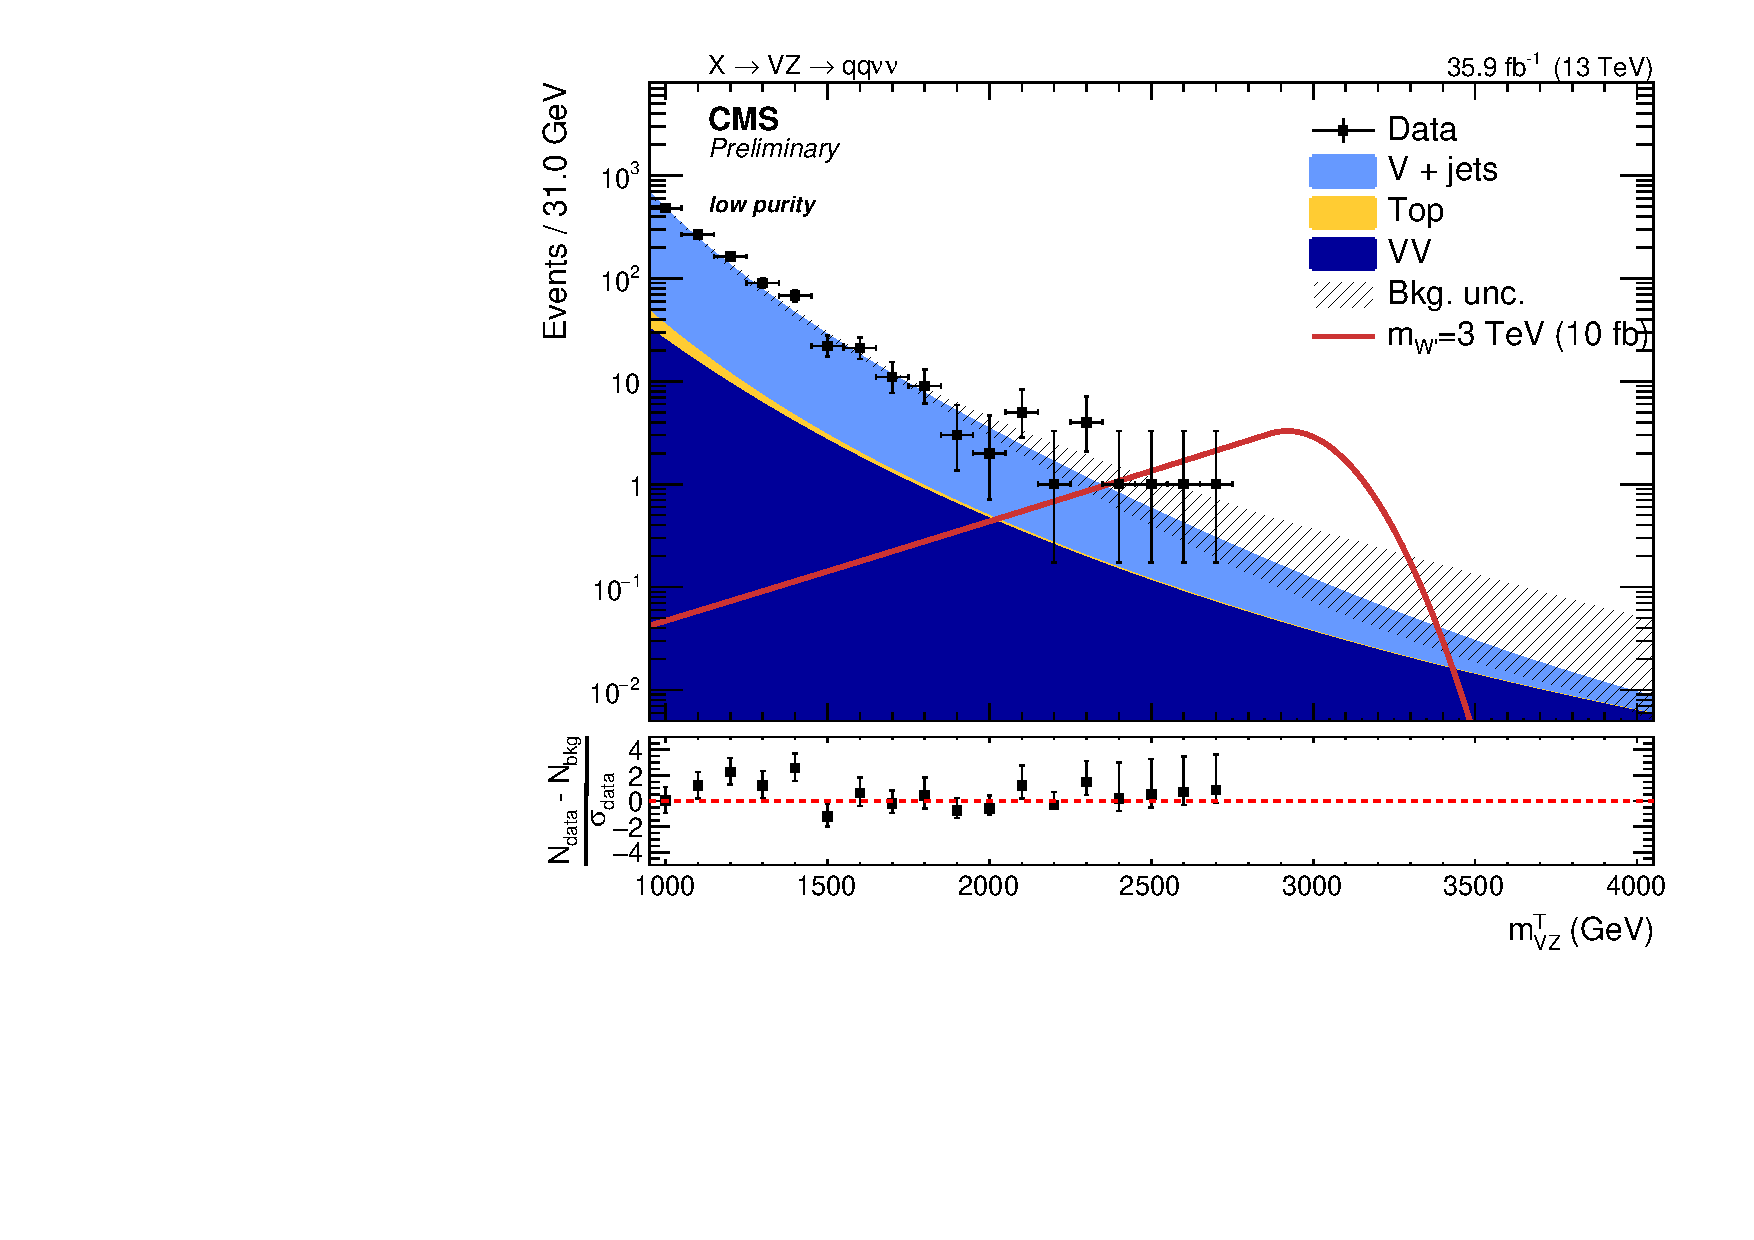
\includegraphics[width=.495\textwidth]{v9/plotsAlpha/XVZnnlp/XVZnnlp_XWZInv_BkgSR.pdf}
    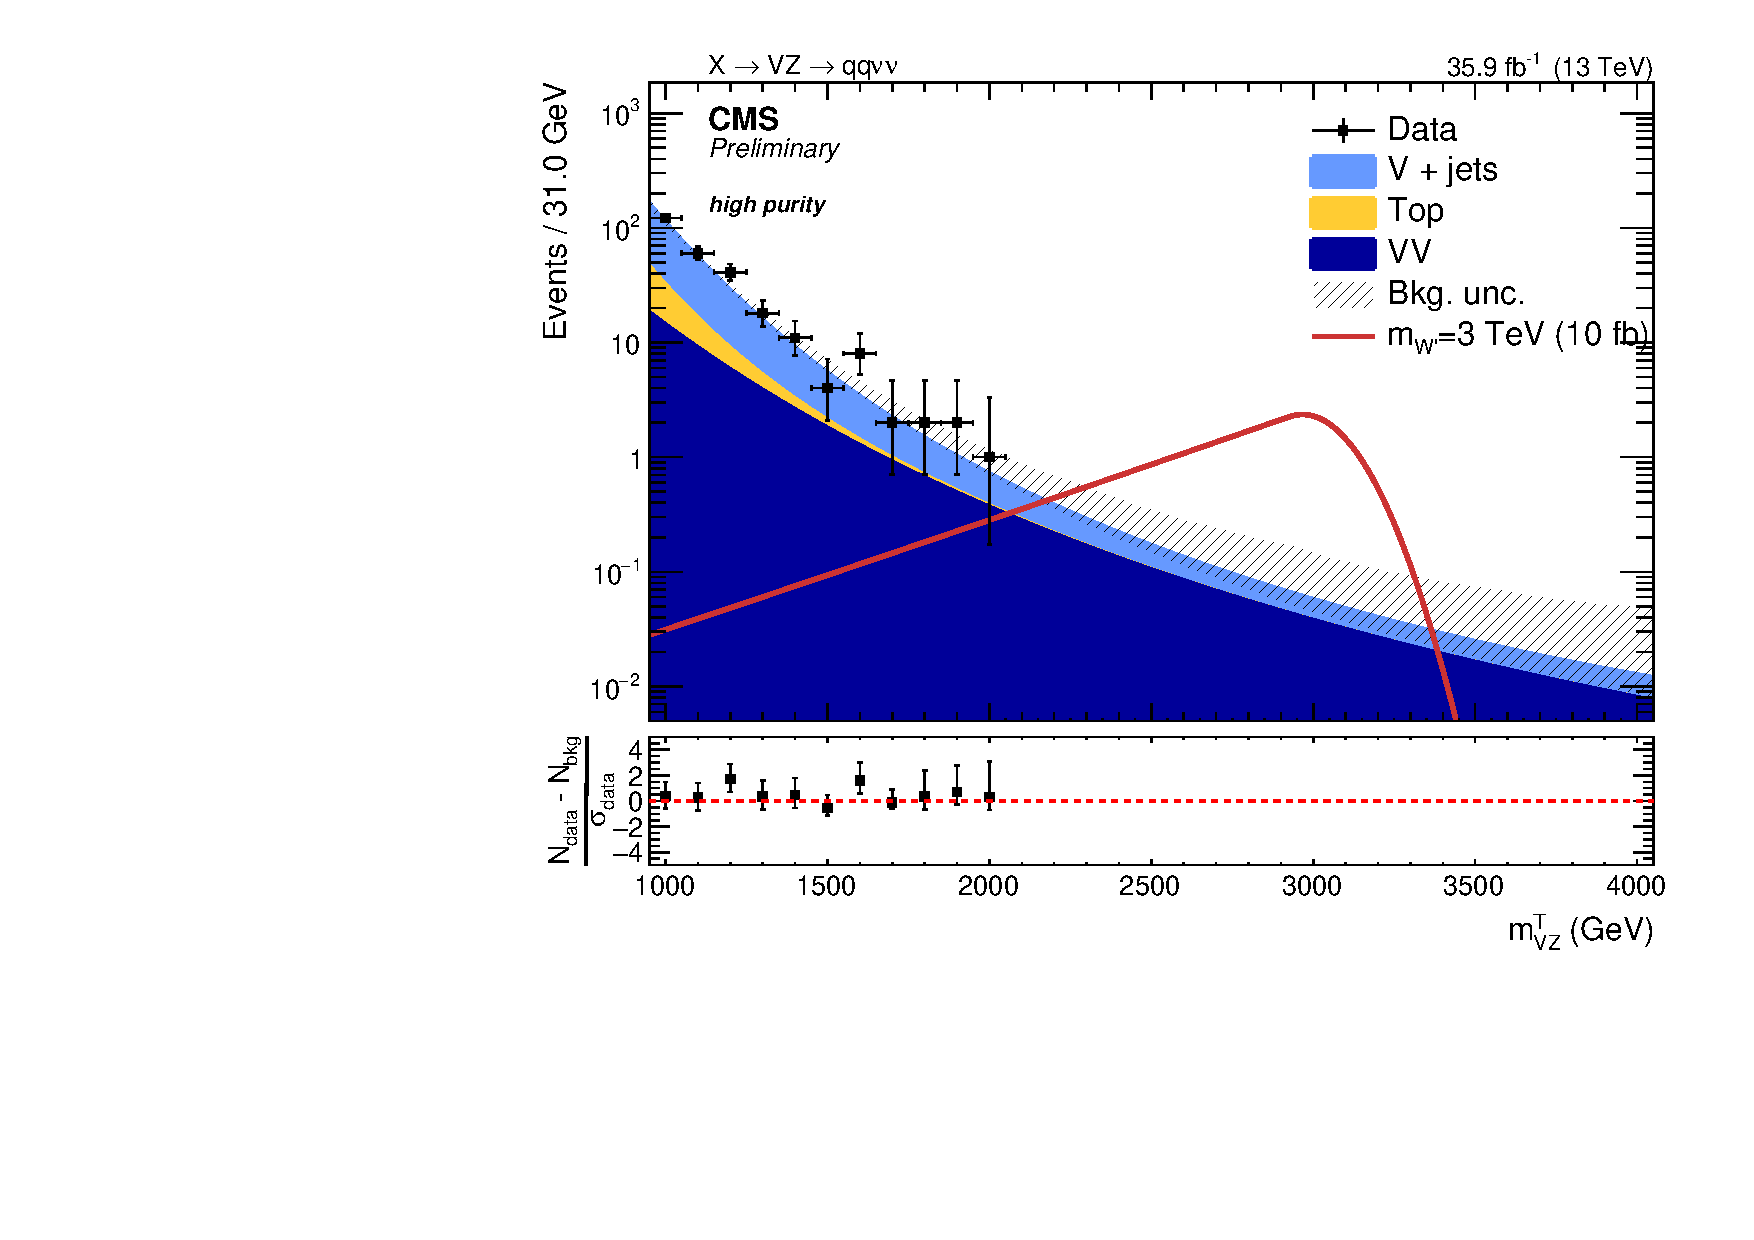
\includegraphics[width=.495\textwidth]{v9/plotsAlpha/XVZnnhp/XVZnnhp_XWZInv_BkgSR.pdf}
  \caption{Expected background with the $\alpha$ method in the low- (left) and high-purity category (right), compared to observations (black dots) and a signal hypotesis of a spin-1 $W^{'}$ of mass 3 \TeV.}
  \label{fig:XVZnn_Exp}
\end{figure}

\clearpage

\subsection{Alpha method validation}

As a validation of the $\alpha$-ratio method described in this Section, a closure test is performed on data. Instead of predicting the background in the real \V SR form both the lower and the upper jet mass sidebands, the SB and SR are redefined for the purposes of this test. 

The low sideband is splitted in two sub-regions: $30-50~\GeV$ (LSB) and $50-65~\GeV$ (SR). The first is considered as the low sideband for the purpose of this test, while the latter is exploited as a pseudo-signal region (and thus not kept blind). The high sideband is instead effectively used in the fit without any modifications with respect to the standard $\alpha$-ratio method.
With this configuration, the prediction of the background in the SR region is estimated from the fit to the LSB region and the high-sidebands, and checked with data for both shape and normalization.

In Figure~\ref{fig:alphaClosure} and Table~\ref{tab:alphaClosure}, the predicted shapes and normalizations are compared to the observed ones in data. 
A good overall agreement both in normalization and shape is obtained. There is a bit of tension in normalization for high-purity category, due to an upper fluctuation in data around 60 \GeV.
This cross check confirms that the method to extract the \V+jets background is reliable and can be used to model the background in the search for potential excesses in the signal region defined in the analysis.

%Comments about not perfect agreement

%[FOLLOWING TABLE-PLOTS: before pre-approval, with ErfExpGaus as main V+jet function for HP]

%\begin{table}[!htb]
%  \begin{center}
%    \begin{tabular}{cc|cc}
%      region & category & Expected & Observed \\
%      \hline
%      SB & $2\nu$, low-purity & $1841.3 \pm 45.7$ & $1793$ \\
%      SR & $2\nu$, low-purity & $529.9 \pm 37.8$ & $521$ \\
%      \hline
%      SB & $2\nu$, high-purity & $728.7 \pm 81.3$ & $725$ \\
%      SR & $2\nu$, high-purity & $47.0 \pm 74.9$ & $49$ \\
%      \hline
%    \end{tabular}
%  \end{center}
%  \caption{Expected and observed background yield in the SR jet mass region ($ 50 < m_j < 65\GeV$), predicted from the LSB one ($30 < m_j < 50\GeV$) and high-sideband ($m_j > 135~\GeV$).}\label{tab:alphaClosure}
%\end{table}

%\begin{figure}[!htb]
%  \centering
%    \includegraphics[width=.495\textwidth]{v9/plotsAlphaExtPt035/XVZnnlp/XVZnnlp_JetMass.pdf}
%    \includegraphics[width=.495\textwidth]{v9/plotsAlphaExtPt035/XVZnnlp/BkgSR.pdf}%BkgSR.pdf}
%    \\
%    \includegraphics[width=.495\textwidth]{v9/plotsAlphaExtPt035/XVZnnhp/XVZnnhp_JetMass.pdf}
%    \includegraphics[width=.495\textwidth]{v9/plotsAlphaExtPt035/XVZnnhp/BkgSR.pdf}%BkgSR.pdf}
%  \caption{Top: fit to the $m_j$ spectrum in data in the sideband defined for the Alpha method validation in the low-purity category: LSB ($30 < m_j < 50\GeV$) and high-sideband ($m_j > 135~\GeV$). Bottom: fit to the $m_j$ spectrum in data in the sideband defined for the Alpha method validation in the high-purity category: LSB ($30 < m_j < 50\GeV$) and high-sideband ($m_j > 135~\GeV$). Both the signal region and the Higgs regions are kept blind, while the pseudo-signal is shown in the SR region ($50 < m_j < 65\GeV$).}
%  \label{fig:alphaClosure}
%\end{figure}

%[FOLLOWING TABLE-PLOTS: after pre-approval, with ExpGaus as main V+jet function for HP]

\begin{table}[!htb]
  \begin{center}
    \begin{tabular}{cc|cc}
      region & category & Expected & Observed \\
      \hline
      SB & $2\nu$, low-purity & $1841.3 \pm 45.7$ & $1793$ \\
      SR & $2\nu$, low-purity & $529.9 \pm 37.8$ & $521$ \\
      \hline
      SB & $2\nu$, high-purity & $728.5 \pm 29.9$ & $725$ \\
      SR & $2\nu$, high-purity & $39.3 \pm 5.2$ & $49$ \\
      \hline
    \end{tabular}
  \end{center}
  \caption{Expected and observed background yield in the SR jet mass region ($ 50 < m_j < 65\GeV$), predicted from the LSB one ($30 < m_j < 50\GeV$) and high-sideband ($m_j > 135~\GeV$).}\label{tab:alphaClosure}
\end{table}

\begin{figure}[!htb]
  \centering
    \includegraphics[width=.495\textwidth]{v9/plotsAlphaExt/XVZnnlp/XVZnnlp_JetMass.pdf}
    \includegraphics[width=.495\textwidth]{v9/plotsAlphaExt/XVZnnlp/BkgSR.pdf}%BkgSR.pdf}
    \\
    \includegraphics[width=.495\textwidth]{v9/plotsAlphaExt/XVZnnhp/XVZnnhp_JetMass.pdf}
    \includegraphics[width=.495\textwidth]{v9/plotsAlphaExt/XVZnnhp/BkgSR.pdf}%BkgSR.pdf}
  \caption{Top: fit to the $m_j$ spectrum in data in the sideband defined for the Alpha method validation in the low-purity category: LSB ($30 < m_j < 50\GeV$) and high-sideband ($m_j > 135~\GeV$). Bottom: fit to the $m_j$ spectrum in data in the sideband defined for the Alpha method validation in the high-purity category: LSB ($30 < m_j < 50\GeV$) and high-sideband ($m_j > 135~\GeV$). Both the signal region and the Higgs regions are kept blind, while the pseudo-signal is shown in the SR region ($50 < m_j < 65\GeV$).}
  \label{fig:alphaClosure}
\end{figure}


\clearpage

\subsection{Signal modeling}

The simulated signal mass points are fitted in the SR with an empiric function in order to be able to perform an unbinned likelihood fit for the signal extraction. 


% The function chosen to model the signal is the \emph{Gaussian}, which consists in a gaussian core and a power function that describes the low-end tail, below a certain threshold.

The function chosen to model the signal samples is a \emph{Crystal ball} function, which is composed by a gaussian-like peak plus a tail towards lower values. Both spin-2 and spin-1 signal samples are fitted.

%[FIXME: plots and fits in this section are obtained only for Bulk Graviton samples]

\begin{figure}[!htb]
  \centering
    \includegraphics[width=.32\textwidth]{v9/plotsAlphaPt035/XVZnnlp/XZZInv_M1000.pdf}
    \includegraphics[width=.32\textwidth]{v9/plotsAlphaPt035/XVZnnlp/XZZInv_M1200.pdf}
    \includegraphics[width=.32\textwidth]{v9/plotsAlphaPt035/XVZnnlp/XZZInv_M1400.pdf}
     \\
    \includegraphics[width=.32\textwidth]{v9/plotsAlphaPt035/XVZnnlp/XZZInv_M1600.pdf}
    \includegraphics[width=.32\textwidth]{v9/plotsAlphaPt035/XVZnnlp/XZZInv_M1800.pdf}
    \includegraphics[width=.32\textwidth]{v9/plotsAlphaPt035/XVZnnlp/XZZInv_M2000.pdf}
     \\
    \includegraphics[width=.32\textwidth]{v9/plotsAlphaPt035/XVZnnlp/XZZInv_M2500.pdf}
    \includegraphics[width=.32\textwidth]{v9/plotsAlphaPt035/XVZnnlp/XZZInv_M3000.pdf}
    \includegraphics[width=.32\textwidth]{v9/plotsAlphaPt035/XVZnnlp/XZZInv_M3500.pdf}
     \\
    \includegraphics[width=.32\textwidth]{v9/plotsAlphaPt035/XVZnnlp/XZZInv_M4000.pdf}
    \includegraphics[width=.32\textwidth]{v9/plotsAlphaPt035/XVZnnlp/XZZInv_M4500.pdf}
  \caption{Fit to the spin-2 (Bulk Graviton) signal samples in the low-purity category.}
  \label{fig:XVZnnlp_Signal}
\end{figure}


\begin{figure}[!htb]
  \centering
    \includegraphics[width=.32\textwidth]{v9/plotsAlphaPt035/XVZnnhp/XZZInv_M1000.pdf}
    \includegraphics[width=.32\textwidth]{v9/plotsAlphaPt035/XVZnnhp/XZZInv_M1200.pdf}
    \includegraphics[width=.32\textwidth]{v9/plotsAlphaPt035/XVZnnlp/XZZInv_M1400.pdf}
     \\
    \includegraphics[width=.32\textwidth]{v9/plotsAlphaPt035/XVZnnhp/XZZInv_M1600.pdf}
    \includegraphics[width=.32\textwidth]{v9/plotsAlphaPt035/XVZnnhp/XZZInv_M1800.pdf}
    \includegraphics[width=.32\textwidth]{v9/plotsAlphaPt035/XVZnnhp/XZZInv_M2000.pdf}
     \\
    \includegraphics[width=.32\textwidth]{v9/plotsAlphaPt035/XVZnnhp/XZZInv_M2500.pdf}
    \includegraphics[width=.32\textwidth]{v9/plotsAlphaPt035/XVZnnhp/XZZInv_M3000.pdf}
    \includegraphics[width=.32\textwidth]{v9/plotsAlphaPt035/XVZnnhp/XZZInv_M3500.pdf}
     \\
    \includegraphics[width=.32\textwidth]{v9/plotsAlphaPt035/XVZnnhp/XZZInv_M4000.pdf}
    \includegraphics[width=.32\textwidth]{v9/plotsAlphaPt035/XVZnnhp/XZZInv_M4500.pdf}
  \caption{Fit to the spin-2 (Bulk Graviton) signal samples in the high-purity category.}
  \label{fig:XVZnnhp_Signal}
\end{figure}

\begin{figure}[!htb]
  \centering
    \includegraphics[width=.32\textwidth]{v9/plotsAlphaPt035/XVZnnlp/XWZInv_M1000.pdf}
    \includegraphics[width=.32\textwidth]{v9/plotsAlphaPt035/XVZnnlp/XWZInv_M1200.pdf}
    \includegraphics[width=.32\textwidth]{v9/plotsAlphaPt035/XVZnnlp/XWZInv_M1400.pdf}
     \\
    \includegraphics[width=.32\textwidth]{v9/plotsAlphaPt035/XVZnnlp/XWZInv_M1600.pdf}
    \includegraphics[width=.32\textwidth]{v9/plotsAlphaPt035/XVZnnlp/XWZInv_M1800.pdf}
    \includegraphics[width=.32\textwidth]{v9/plotsAlphaPt035/XVZnnlp/XWZInv_M2000.pdf}
     \\
    \includegraphics[width=.32\textwidth]{v9/plotsAlphaPt035/XVZnnlp/XWZInv_M2500.pdf}
    \includegraphics[width=.32\textwidth]{v9/plotsAlphaPt035/XVZnnlp/XWZInv_M3000.pdf}
    \includegraphics[width=.32\textwidth]{v9/plotsAlphaPt035/XVZnnlp/XWZInv_M3500.pdf}
     \\
    \includegraphics[width=.32\textwidth]{v9/plotsAlphaPt035/XVZnnlp/XWZInv_M4000.pdf}
    \includegraphics[width=.32\textwidth]{v9/plotsAlphaPt035/XVZnnlp/XWZInv_M4500.pdf}
  \caption{Fit to the spin-1 ($W^{'}$) signal samples in the low-purity category.}
  \label{fig:XWZnnlp_Signal}
\end{figure}


\begin{figure}[!htb]
  \centering
    \includegraphics[width=.32\textwidth]{v9/plotsAlphaPt035/XVZnnhp/XWZInv_M1000.pdf}
    \includegraphics[width=.32\textwidth]{v9/plotsAlphaPt035/XVZnnhp/XWZInv_M1200.pdf}
    \includegraphics[width=.32\textwidth]{v9/plotsAlphaPt035/XVZnnlp/XWZInv_M1400.pdf}
     \\
    \includegraphics[width=.32\textwidth]{v9/plotsAlphaPt035/XVZnnhp/XWZInv_M1600.pdf}
    \includegraphics[width=.32\textwidth]{v9/plotsAlphaPt035/XVZnnhp/XWZInv_M1800.pdf}
    \includegraphics[width=.32\textwidth]{v9/plotsAlphaPt035/XVZnnhp/XWZInv_M2000.pdf}
     \\
    \includegraphics[width=.32\textwidth]{v9/plotsAlphaPt035/XVZnnhp/XWZInv_M2500.pdf}
    \includegraphics[width=.32\textwidth]{v9/plotsAlphaPt035/XVZnnhp/XWZInv_M3000.pdf}
    \includegraphics[width=.32\textwidth]{v9/plotsAlphaPt035/XVZnnhp/XWZInv_M3500.pdf}
     \\
    \includegraphics[width=.32\textwidth]{v9/plotsAlphaPt035/XVZnnhp/XWZInv_M4000.pdf}
    \includegraphics[width=.32\textwidth]{v9/plotsAlphaPt035/XVZnnhp/XWZInv_M4500.pdf}
  \caption{Fit to the spin-1 ($W^{'}$) signal samples in the high-purity category.}
  \label{fig:XWZnnhp_Signal}
\end{figure}


\clearpage

\subsubsection{Signal parametrization}

The signal is parametrized by interpolating the fitted parameters separately for each channel in order to have a continous variation of the signal shape for every possible \mX value within the range. A linear fit is performed on the mean and the width of the Gaussian. The interpolations are shown in Fig.~\ref{fig:XZZ_SignalShapeLP}-~\ref{fig:XZZ_SignalShapeHP} for the spin-2 signal model, and in Fig.~\ref{fig:XWZ_SignalShapeLP}-~\ref{fig:XWZ_SignalShapeHP} for the spin-1 signal model. Shape systematic uncertainties, as described in section~\ref{sec:uncertainties}, are taken into account while describing the mean and sigma of the gaussian core, and they are related to the effects of the jet mass scale and resolution. Other shape parameters describing the tails of the Crystal Ball are fitted as 3rd degree polynomial.

%[FIXME: since some Crystal Ball fits are partially failing, some parameters have awkward uncertainties, so the polynomial function is off, especially for the exponential slope parameter (bottom right). In this case, the SPLINE approach is chosen.]

\begin{figure}[!htb]
  \centering
    \includegraphics[width=.95\textwidth]{v9/plotsAlphaPt035/XVZnnlp/XZZInv_SignalShape.pdf}
  \caption{Interpolation of the fitted parameters as a function of the generated mass \mtVZ, for a spin-2 (Bulk Graviton) signal hypothesis, low-purity category.}
  \label{fig:XZZ_SignalShapeLP}
\end{figure}

\begin{figure}[!htb]
  \centering
    \includegraphics[width=.95\textwidth]{v9/plotsAlphaPt035/XVZnnhp/XZZInv_SignalShape.pdf}

  \caption{Interpolation of the fitted parameters as a function of the generated mass \mtVZ, for a spin-2 (Bulk Graviton) signal hypothesis, high-purity category.}
  \label{fig:XZZ_SignalShapeHP}
\end{figure}

\begin{figure}[!htb]
  \centering
    \includegraphics[width=.95\textwidth]{v9/plotsAlphaPt035/XVZnnlp/XWZInv_SignalShape.pdf}
  \caption{Interpolation of the fitted parameters as a function of the generated mass \mtVZ, for a spin-1 ($W^{'}$) signal hypothesis, low-purity category.}
  \label{fig:XWZ_SignalShapeLP}
\end{figure}

\begin{figure}[!htb]
  \centering
    \includegraphics[width=.95\textwidth]{v9/plotsAlphaPt035/XVZnnhp/XWZInv_SignalShape.pdf}

  \caption{Interpolation of the fitted parameters as a function of the generated mass \mtVZ, for a spin-1 ($W^{'}$) signal hypothesis, high-purity category.}
  \label{fig:XWZ_SignalShapeHP}
\end{figure}


The normalization of the signal samples is extrapolated from the fitted integral of the Gaussian functions. The points are then connected with a line, in order to have an acceptable description of the normalization as a function of \mtVZ.
The interpolations are shown in Fig.~\ref{fig:XZZ_SignalNorm} for the spin-2 signal model, in Fig.~\ref{fig:XWZ_SignalNorm} for the spin-1 signal model.% and Fig.~\ref{fig:XWZ_SignalNorm}.

\begin{figure}[!htb]
  \centering
    \includegraphics[width=.495\textwidth]{v9/plotsAlphaPt035/XVZnnlp/XZZInv_SignalNorm.pdf}
    \includegraphics[width=.495\textwidth]{v9/plotsAlphaPt035/XVZnnhp/XZZInv_SignalNorm.pdf}
  \caption{Interpolation of the signal normalization as a function of the generated mass \mtVZ, for a spin-2 (Bulk Graviton) signal hypothesis. From left to right: low-purity, high-purity.}
  \label{fig:XZZ_SignalNorm}
\end{figure}

\begin{figure}[!htb]
  \centering
    \includegraphics[width=.495\textwidth]{v9/plotsAlphaPt035/XVZnnlp/XWZInv_SignalNorm.pdf}
    \includegraphics[width=.495\textwidth]{v9/plotsAlphaPt035/XVZnnhp/XWZInv_SignalNorm.pdf}
  \caption{Interpolation of the signal normalization as a function of the generated mass \mtVZ, for a spin-1 ($W^{'}$) signal hypothesis. From left to right: low-purity, high-purity.}
  \label{fig:XWZ_SignalNorm}
\end{figure}

\begin{figure}[!htb]
  \centering
    \includegraphics[width=.495\textwidth]{v9/plotsAlphaPt035/XVZnnlp/XZZInv_Signal.pdf}
    \includegraphics[width=.495\textwidth]{v9/plotsAlphaPt035/XVZnnhp/XZZInv_Signal.pdf}
  \caption{Interpolation of the signal as a function of the generated mass \mtVZ, for a spin-2 (Bulk Graviton) signal hypothesis with an arbitrary cross section of 1 \pb in the low- (left) and high-purity category (right).}
  \label{fig:XZZInv_Signal}
\end{figure}

\begin{figure}[!htb]
  \centering
    \includegraphics[width=.495\textwidth]{v9/plotsAlphaPt035/XVZnnlp/XWZInv_Signal.pdf}
    \includegraphics[width=.495\textwidth]{v9/plotsAlphaPt035/XVZnnhp/XWZInv_Signal.pdf}
  \caption{Interpolation of the signal as a function of the generated mass \mtVZ, for a spin-1 ($W^{'}$) signal hypothesis with an arbitrary cross section of 1 \pb in the low- (left) and high-purity category (right).}
  \label{fig:XWZInv_Signal}
\end{figure}

%\begin{table}[!htb]
%  \begin{center}
%    \begin{tabular}{c|cc|cc}
%      Channel & \multicolumn{2}{c}{Mean} & \multicolumn{2}{c}{Width} \\
%      & q & m & q & m \\
%      \hline
%XVZeelp	&	7.35	&	0.990	&	19.53	&	0.0437	\\
%XVZeehp	&	-1.56	&	0.993	&	18.8	&	0.0407	\\
%XVZmmlp	&	20.2	&	0.980	&	37.1	&	0.0303	\\
%XVZmmhp	&	5.24	&	0.985	&	9.84	&	0.0452	\\
%      \hline
%    \end{tabular}

%    \begin{tabular}{c|cccccc|ccc}
%      Channel & \multicolumn{6}{c}{5 order polynomial} \\
%      & p0 & p1 & p2 & p3 & p4 & p5 \\
%      \hline
%XVZeelp	&	-6.063527e+01 & 1.275113e-01 & 4.505761e-04 & -3.471543e-07 & 9.135174e-11 & -8.149492e-15 \\
%XVZeehp	&	-5.737452e+02 & 2.076764e+00 & -1.156219e-03 & 2.833294e-07 & -3.072449e-11 & 1.081726e-15 \\
%XVZmmlp	&	-1.861969e+03 & 5.243766e+00 & -4.499331e-03 & 1.792072e-06 & -3.353744e-10 & 2.379620e-14 \\
%XVZmmhp	&	-1.522785e+03 & 5.343553e+00 & -4.323340e-03 & 1.583020e-06 & -2.738677e-10 & 1.813525e-14 \\
%      \hline
%    \end{tabular}
%  \end{center}
%  \caption{Parameters of the functions used to parametrize the signal.}\label{tab:Parameters}
%\end{table}

%   'XVZeelp' : {'mean' : [7.359275e+00, 9.905230e-01], 'sigma' : [1.931214e+01, 4.517162e-02], 'alpha' : [2.000000e+00, 0.], 'slope' : [1.000000e+00, 0.], 'norm' : [-6.063527e+01, 1.275113e-01, 4.505761e-04, -3.471543e-07, 9.135174e-11, -8.149492e-15, 0., 0., 0., 0.]},
%   'XVZeehp' : {'mean' : [-1.563159e+00, 9.933155e-01], 'sigma' : [1.883610e+01, 3.034543e-02], 'alpha' : [2.000000e+00, 0.], 'slope' : [1.000000e+00, 0.], 'norm' : [-5.737452e+02, 2.076764e+00, -1.156219e-03, 2.833294e-07, -3.072449e-11, 1.081726e-15, 0., 0., 0., 0.]},
%   'XVZmmlp' : {'mean' : [2.021176e+01, 9.804471e-01], 'sigma' : [3.707876e+01, 4.073031e-02], 'alpha' : [2.000000e+00, 0.], 'slope' : [1.000000e+00, 0.], 'norm' : [-1.861969e+03, 5.243766e+00, -4.499331e-03, 1.792072e-06, -3.353744e-10, 2.379620e-14, 0., 0., 0., 0.]},
%   'XVZmmhp' : {'mean' : [5.240178e+00, 9.850675e-01], 'sigma' : [9.848569e+00, 4.367182e-02], 'alpha' : [2.000000e+00, 0.], 'slope' : [1.000000e+00, 0.], 'norm' : [-1.522785e+03, 5.343553e+00, -4.323340e-03, 1.583020e-06, -2.738677e-10, 1.813525e-14, 0., 0., 0., 0.]},

\clearpage

\clearpage

